\documentclass[10pt]{beamer}

% Beamer style
%\usetheme[secheader]{Madrid}
% \usetheme{CambridgeUS}
\useoutertheme{infolines}
\usecolortheme[rgb={0.65,0.15,0.25}]{structure}
% \usefonttheme[onlymath]{serif}
\beamertemplatenavigationsymbolsempty
%\AtBeginSubsection

% Packages
%\usepackage[french]{babel}
\usepackage[latin1]{inputenc}
\usepackage{color}
\usepackage{xspace}
\usepackage{dsfont, stmaryrd}
\usepackage{amsmath, amsfonts, amssymb, MnSymbol}
\usepackage{epsfig}
\usepackage{url}
\usepackage{/home/robin/LATEX/Biblio/astats}
%\usepackage[all]{xy}
\usepackage{graphicx}

% Commands
\definecolor{darkred}{rgb}{0.65,0.15,0.25}
\newcommand{\emphase}[1]{\textcolor{darkred}{#1}}
% \newcommand{\emphase}[1]{{#1}}
\newcommand{\paragraph}[1]{\textcolor{darkred}{#1}}
\newcommand{\refer}[1]{{\small{\textcolor{gray}{{[\cite{#1}]}}}}}
% \newcommand{\Refer}[1]{{\small{\textcolor{gray}{{[#1]}}}}}
\renewcommand{\newblock}{}

% Symbols
\newcommand{\Abf}{{\bf A}}
\newcommand{\Beta}{\text{B}}
\newcommand{\Bcal}{\mathcal{B}}
\newcommand{\BIC}{\text{BIC}}
\newcommand{\Ccal}{\mathcal{C}}
\newcommand{\dd}{\text{~d}}
\newcommand{\dbf}{{\bf d}}
\newcommand{\Dcal}{\mathcal{D}}
\newcommand{\Esp}{\mathbb{E}}
\newcommand{\Ebf}{{\bf E}}
\newcommand{\Ecal}{\mathcal{E}}
\newcommand{\Gcal}{\mathcal{G}}
\newcommand{\Gam}{\mathcal{G}\text{am}}
\newcommand{\Hcal}{\mathcal{H}}
\newcommand{\Ibb}{\mathbb{I}}
\newcommand{\Ibf}{{\bf I}}
\newcommand{\ICL}{\text{ICL}}
\newcommand{\Cov}{\mathbb{C}\text{ov}}
\newcommand{\Corr}{\mathbb{C}\text{orr}}
\newcommand{\Var}{\mathbb{V}}
\newcommand{\Vsf}{\mathsf{V}}
\newcommand{\pen}{\text{pen}}
\newcommand{\Fcal}{\mathcal{F}}
\newcommand{\Hbf}{{\bf H}}
\newcommand{\Jcal}{\mathcal{J}}
\newcommand{\Kbf}{{\bf K}}
\newcommand{\Lcal}{\mathcal{L}}
\newcommand{\Mcal}{\mathcal{M}}
\newcommand{\mbf}{{\bf m}}
\newcommand{\mum}{\mu(\mbf)}
\newcommand{\Ncal}{\mathcal{N}}
\newcommand{\Nbf}{{\bf N}}
\newcommand{\Nm}{N(\mbf)}
\newcommand{\Ocal}{\mathcal{O}}
\newcommand{\Obf}{{\bf 0}}
\newcommand{\Omegas}{\underset{s}{\Omega}}
\newcommand{\Pbf}{{\bf P}}
\newcommand{\Pt}{\widetilde{P}}
\newcommand{\pt}{\widetilde{p}}
\newcommand{\Pcal}{\mathcal{P}}
\newcommand{\Qcal}{\mathcal{Q}}
\newcommand{\Rbb}{\mathbb{R}}
\newcommand{\Rcal}{\mathcal{R}}
\newcommand{\Scal}{\mathcal{S}}
\newcommand{\Tcal}{\mathcal{T}}
\newcommand{\Ucal}{\mathcal{U}}
\newcommand{\Vcal}{\mathcal{V}}
\newcommand{\BP}{\text{BP}}
\newcommand{\EM}{\text{EM}}
\newcommand{\VEM}{\text{VEM}}
\newcommand{\VBEM}{\text{VBEM}}
\newcommand{\cst}{\text{cst}}
\newcommand{\obs}{\text{obs}}
\newcommand{\ra}{\emphase{\mathversion{bold}{$\rightarrow$}~}}
%\newcommand{\transp}{\text{{\tiny $\top$}}}
\newcommand{\transp}{\text{{\tiny \mathversion{bold}{$\top$}}}}
\newcommand{\logit}{\text{logit}\xspace}
\newcommand{\SBMreg}{\text{SBM-reg}\xspace}

% Directory
\newcommand{\fignet}{/home/robin/RECHERCHE/RESEAUX/EXPOSES/FIGURES}
\newcommand{\figbayes}{/home/robin/RECHERCHE/BAYES/EXPOSES/FIGURES}


%====================================================================
%====================================================================

%====================================================================
%====================================================================
\begin{document}
%====================================================================
%====================================================================

%====================================================================
\title[Bayesian GOF for logistic graphs]{Goodness of fit for graph logistic regression: \\
  a (variational) Bayes approach}

\author[S. Robin]{S. Robin \\ ~\\
  Joint work with S. Donnet P. Latouche, S. Ouadah.
  }

\institute[INRA / AgroParisTech]{~ \\%INRA / AgroParisTech \\
%   \vspace{-.1\textwidth}
  \begin{tabular}{ccc}
    
\includegraphics[height=.05\textheight]{\fignet/LogoINRA-Couleur} & 
    \hspace{.02\textheight} &
    
\includegraphics[height=.06\textheight]{\fignet/logagroptechsolo} % & 
%     \hspace{.02\textheight} &
%     
\includegraphics[height=.09\textheight]{\fignet/logo-ssb}
    \\ 
  \end{tabular} \\
  \bigskip
  }

\date[Dec. 2017, Leiden]{Bayes Club, Dec. 2017, Leiden}

%====================================================================
%====================================================================
\maketitle
%====================================================================

%====================================================================
%====================================================================
\section{Motivating example}
%====================================================================
\frame{\frametitle{Tree interaction network} 

  \paragraph{Data.}
  \begin{itemize}
    \item $n$ tree species
    \item network
    $$
    i \sim j \quad \Leftrightarrow \quad \text{species $i$ and $j$ share at least one parasite}
    $$
    \item $d$ covariates: genetic, phylogenetic and geographic distance between each pair of species
  \end{itemize}
  
  \bigskip 
  \paragraph{Questions.}
  \begin{itemize}
    \item Do covariates explain why species interact?
    \item Do the covariates explain the whole topology of the network?
    \item If not, how to depict the residual structure of the network?
  \end{itemize}

}

%====================================================================
\frame{\frametitle{Tree network: the data} 

  \begin{tabular}{cc}
    \hspace{-.05\textwidth}
    \begin{tabular}{c}
	 \begin{tabular}{cc}
	   \vspace{-.025\textheight}
	   Genetic dist. 
	   &
	   Geographic dist. \\
	   \includegraphics[width=.3\textwidth]{../FIGURES/FigSBMreg-Tree-Genetic} 
	   & 
	   \includegraphics[width=.3\textwidth]{../FIGURES/FigSBMreg-Tree-Geographic} \\
	   \vspace{-.075\textheight}
	   Taxonomic dist. 
	   &
	   Network
	   \\ ~\\
	   \includegraphics[width=.3\textwidth]{../FIGURES/FigSBMreg-Tree-Taxonomic}
	   &
	   \includegraphics[width=.3\textwidth]{../FIGURES/FigSBMreg-Tree-BinaryAdjacency} \\
	 \end{tabular}
    \end{tabular}
    & 
    \hspace{-.15\textwidth}
    \begin{tabular}{c}
	 Network \\
	 \includegraphics[width=.4\textwidth]{../FIGURES/FigSBMreg-Tree-BinaryNetwork} 
    \end{tabular}
  \end{tabular}
}

%====================================================================
%====================================================================
\section{\SBMreg model}
\frame{\frametitle{Outline} \tableofcontents[currentsection]}
%====================================================================
\frame{\frametitle{Statistical model} 

  \paragraph{Aim}
  \begin{enumerate}
   \item Account for the effect of (edge) covariates
   \item Account for some network-structured residual
  \end{enumerate}

  \bigskip
  \paragraph{Idea:} combine two classical models
  \begin{enumerate}
   \item Logistic regression: $(Y_{ij})_{i<j}$ indep., 
   $$
   \logit \, P(Y_{ij} = 1) = x_{ij}^\intercal \, \beta
   $$
   \item $W$-graph: $ (U_i)_i \text{ iid} \sim \Ucal_{[0, 1]}$, \quad $(Y_{ij})_{i < j}$ indep. $\,|\, (U_i)_i$,  
   $$
  \logit \, P(Y_{ij} = 1 \,|\, U_i, U_j) = \phi(U_i, U_j)
   $$
   $\phi =$ (logit-)graphon function
  \end{enumerate}
}

%====================================================================
\frame{\frametitle{$W$-graph model \refer{LoS06}} 

  \begin{tabular}{cc}
    \hspace{-.05\textwidth}
    \begin{tabular}{p{.5\textwidth}}
    \begin{itemize}
     \item Latent variables:
     $$
     (U_i) \text{ iid } \sim \Ucal_{[0, 1]},
     $$
     \item Graphon function:
     $$
     \phi(u, v): [0, 1]^2 \mapsto [0, 1]
     $$
     Edges:
     $$
     P(Y_{ij} = 1|U_i, U_j) = \phi(U_i, U_j)
     $$    
    \end{itemize} \\~ \\~ \\~ 
    \end{tabular}
    & 
    \hspace{-.05\textwidth}
    \begin{tabular}{p{.5\textwidth}}
	 Graphon $\phi(u, v)$ \\
      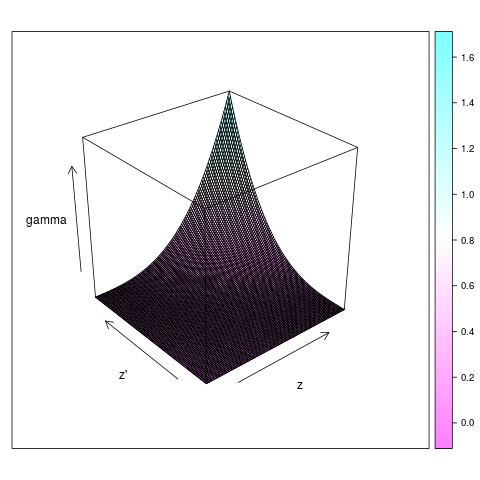
\includegraphics[width=.45\textwidth]{../FIGURES/FigCLADAG-W-graphon} 
    \end{tabular}
  \end{tabular}
}

%====================================================================
\frame{\frametitle{Stochastic block-model \refer{Hol79,NoS01}} 

  \begin{tabular}{cc}
    \hspace{-.05\textwidth}
    \begin{tabular}{p{.5\textwidth}}
	 \vspace{-.3\textheight}
	 \begin{itemize}
	 \item Latent variables:
	 $$
	 (Z_i) \text{ iid } \sim \Mcal(1, \pi)
	 $$
	 \item Blockwise constant graphon:
	 \begin{eqnarray*}
	  	 & & \phi(z, z') \\
	  	 & = & \sum_{k, \ell} \alpha_{k\ell} \Ibb\{z \in B_k, z' \in B_\ell\}
	 \end{eqnarray*}
	 \item Edges:
	 $$
	 P(Y_{ij} = 1|Z_i, Z_j) = \phi(Z_i, Z_j) 
	 $$
	 \end{itemize} \\~ \\~ \\~ 
    \end{tabular}
    & 
    \hspace{-.05\textwidth}
    \begin{tabular}{p{.5\textwidth}}
	 \vspace{.1\textheight}
	 \begin{overprint}
	 \onslide<1>
	 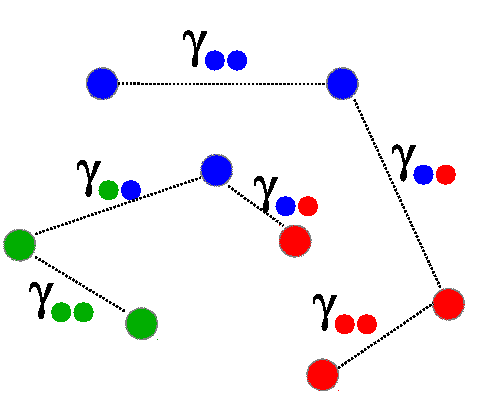
\includegraphics[width=.45\textwidth]{../FIGURES/FigSBM-Model-3-red} 
	 \onslide<2>
	 Graphon function of $SBM_K$ \\ 
	 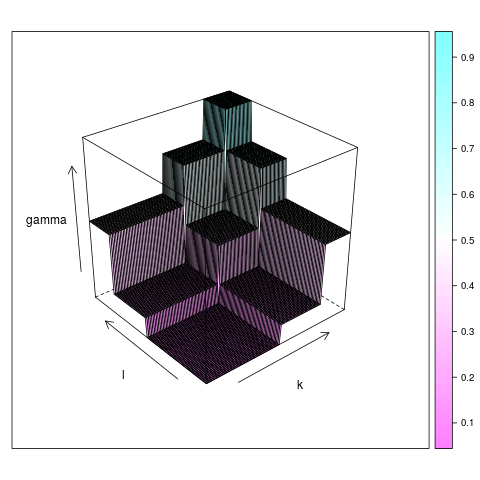
\includegraphics[width=.45\textwidth]{../FIGURES/FigCLADAG-SBM-graphon} 
% 	 \onslide<3>
% 	 VB estimate for $SBM_K$ \refer{LaR16} \\ 
% 	 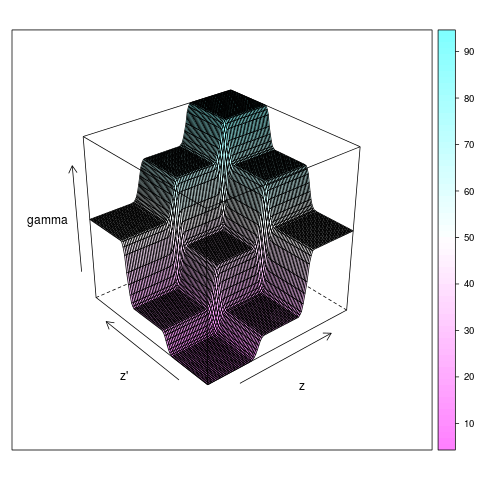
\includegraphics[width=.4475\textwidth]{../FIGURES/FigGraphon-SBM-average} 
	 \end{overprint}
    \end{tabular}
  \end{tabular}
}

%====================================================================
\frame{\frametitle{Proposed model \refer{LRO17}} 

  \paragraph{'Ideal' model:} $(U_i)_i \text{ iid} \sim \Ucal_{[0, 1]}$, \quad $(Y_{ij})_{i < j}$ indep. $\,|\, (U_i)_i$,  
  $$
  \logit \, P(Y_{ij} = 1 \,|\, U_i, U_j) = \underset{\text{covariate effect}}
  {\underbrace{~~ x_{ij}^\intercal \, \beta ~~}} + \underset{\text{residual structure}}
  {\underbrace{\phi(U_i, U_j)}}
  $$
  \ra Fully non-parametric estimation of $\phi$ not easy

  \bigskip \bigskip \pause
  \paragraph{\SBMreg model:} Block-wise constant approximation of $\phi$ \refer{LaR16} \\
  $$
  (Z_i)_i \text{ iid} \sim \Mcal_K(1, \pi), \quad (Y_{ij})_{i < j} \text{ indep. } \,|\,  (Z_i)_i,
  $$

  $$
  \logit \, P(Y_{ij} = 1 \,|\, Z_i, Z_j) = \underset{\text{covariate effect}}
  {\underbrace{~~ x_{ij}^\intercal \, \beta ~~}} + \underset{\text{residual structure}}
  {\underbrace{\alpha_{Z_i, Z_j}}}
  $$
}

%====================================================================
\frame{\frametitle{Full Bayesian model} 

  \begin{tabular}{cc}
    \hspace{-.05\textwidth}
    \begin{tabular}{p{.55\textwidth}}
      \begin{itemize}
      \item $\beta \sim \Ncal(\beta)$: regression coefficients \\ ~
      \item $K \sim P(K)$: number of blocks \\ ~
      \item $\pi \sim \Dcal(\pi\,|\,K)$: block proportions \\ ~
      \item $Z \sim \Mcal(Z\,|\,\pi)$: block memberships \\ ~
      \item $\alpha \sim \Ncal(\alpha\,|\,K)$: block interactions \\ ~
      \item $Y \sim \Bcal(Y\,|\,Z, \alpha, \beta)$: network
      \end{itemize}
    \end{tabular}
    & 
    \hspace{-.05\textwidth}
    \begin{tabular}{p{.5\textwidth}}
    \includegraphics[width=.6\textwidth]{../FIGURES/FigSBMreg-GraphModel2} \\
    \paragraph{Notations:} \\
    $x = (x^\ell_{ij}), Z = (Z_i), Y = (Y_{ij})$, \\
    $\theta = (\beta, \pi, \alpha)$
    \end{tabular}
  \end{tabular}
}

%====================================================================
\frame{\frametitle{Back to the original problem} 

  \paragraph{Questions.}
  \begin{itemize}
    \item Do covariates explain why species interact?
    $$
    p(\beta \,|\, Y)
    $$ \\~
    \item Do the covariates explain the whole topology of the network?
    $$
    p(K = 1 \,|\, Y)
    $$ \\~
    \item If not, how to depict the residual structure of the network?
    $$
    \widehat{\phi}(u, v) = \sum_k P(K = k \,|\,Y) \Esp[\phi(u, v) \,|\, Y, K=k]
    $$
  \end{itemize}
}

%====================================================================
%====================================================================
\section{Variational Bayes inference}
\frame{\frametitle{Outline} \tableofcontents[currentsection]}
%====================================================================
\frame{\frametitle{A reminder on variational Bayes} 

  \paragraph{Aim:} approximate the posterior
  $$
  \pt(\theta) \approx p(\theta \,|\, Y),
  $$
  typically
  $$
  \pt(\cdot) = \arg\min_{q \in \Qcal} KL[q(\cdot) \,||\, p(\cdot\,|\,Y)].
  $$
  
  \bigskip \bigskip 
  \paragraph{Models with hidden variables \refer{BeG03}:} get
  $$
  \pt(\theta, Z) \approx p(\theta, Z \,|\, Y),
  $$
  typically, assume that $\pt(\theta, Z) = \pt_\theta(\theta) \; \pt_Z(Z)$ \ra VB-EM.
}

%====================================================================
\frame{\frametitle{Two examples} 

  \paragraph{Logistic regression \refer{JaJ00}:} $\Qcal = \Ncal$,
  $$
  \beta \sim \Ncal(m, S), \quad Y_i \,|\, \beta \sim \Bcal\left(\frac1{1-e^{x_i^\intercal \beta}}\right):
  \quad 
  \pt(\beta) = \Ncal(\widetilde{m}, \widetilde{S})
  $$
  
  \bigskip 
  \paragraph{SBM \refer{DPR08,GDR12,LaR16}:} $\Qcal = \{\text{factorized distribution}\}$
  $$
  \pt(Z) = \prod_i \pt_i(Z_i)
  $$
  \ra mean-field approximation (R package {\tt mixer} on CRAN)
  
  \bigskip \bigskip 
  Both perform well (both empirical and theoretical arguments)
}

%====================================================================
\frame{\frametitle{VB inference for \SBMreg} 

  \paragraph{VB-EM:} a VB-EM algorithm can be designed \refer{LRO17} to get
  $$
  \pt^K(\theta, Z) = \pt^K_\theta(\theta) \; \pt^K_Z(Z) \approx p(\theta, Z| Y, K)
  $$
  
  \bigskip
  \paragraph{Posterior of $K$:} VB approximation also holds to get \refer{VMR12} 
  $$
  \pt(K) \approx p(K \,|\, Y)
  $$
  
  \bigskip
  \paragraph{Bayesian model averaging} then applies to get, e.g.
  $$
  \pt(\theta) = \sum_k \Pt(K = k) \pt_\theta^k(\theta)
  $$
  
  \bigskip
  \paragraph{R package} {\tt GOFnetwork} (\url{github.com/platouche/gofNetwork})
}

%====================================================================
\frame{\frametitle{Tree network} 


  \begin{tabular}{cc}
    \hspace{-.05\textwidth}
    \begin{tabular}{p{.55\textwidth}}
    \paragraph{Covariate effects:} $\pt(\beta)$ \\
    {\footnotesize
	 \begin{tabular}{lccc}
% 	 & \multicolumn{3}{c|}{VB} \\
	 & genet. & geogr. & taxo. \\ \hline
	 mean & $4.6 \; 10^{-5}$ & $2.3 \; 10^{-1}$ & $-9.0 \; 10^{-1}$ \\ 
% 	 within var. & $2.2 \; 10^{-10}$ & $4.3 \; 10^{-2}$ & \emphase{$1.7 \; 10^{-3}$} \\ 
% 	 between var. & $5.6 \; 10^{-17}$ & $1.2 \; 10^{-6}$ & \emphase{$2.4 \; 10^{-7}$} \\ 
	 st. dev. & $1.5 \; 10^{-5}$ & $2.1 \; 10^{-1}$ & \; $4.2 \; 10^{-2}$ \\ 
	 ratio &  $3.1$ & $1.1$ & $-21$ 
    \end{tabular}
    }

    \bigskip \bigskip \pause
    \paragraph{Goodness of fit:} 
    $$
    \Pt(K = 1) = 4.83 \; 10^{-153} \quad (!!!)
    $$ 
    
    \bigskip \bigskip \pause
    Covariates partially explain the network topology \\ ~
    \end{tabular}
    & 
    \begin{tabular}{p{.5\textwidth}} \pause
    \paragraph{Without covariates:} ~ \\
    \includegraphics[width=.3\textwidth]{../FIGURES/treed0} \\ ~\\ \pause
    \paragraph{Residual:} ~ \\
    \includegraphics[width=.3\textwidth]{../FIGURES/treed3} \\
    \end{tabular}
  \end{tabular}

}

%====================================================================
%====================================================================
\section{Bridge sampling}
\frame{\frametitle{Outline} \tableofcontents[currentsection]}
%====================================================================
\frame{\frametitle{From VB approximation to the true posterior} 

  \paragraph{VBEM} only provides an approximation of the true posterior
  $$
  \pt(\theta) \approx p(\theta|Y),
  $$
  \ra Can we use it to evaluate the true posterior?
  
  \bigskip \bigskip \pause
  \paragraph{First idea = Importance sampling (IS):} $(\theta^m)$ iid $\sim q$, 
  $$
  \widehat{\Esp}[f(\theta) | Y] = \sum_m W^m f(\theta^m), \qquad
  w^m = \frac{p(\theta^m|Y)}{q(\theta^m)}, \qquad
  W^m = \frac{w^m}{\sum_\ell w^\ell}
  $$
  \ra Use $\pt$ as the proposal distribution $q$.
}

%==================================================================== 
\frame{\frametitle{Importance of the proposal} 
 
  Effective sample size $= ESS := \overline{w}^2 / \overline{w^2}$. 
 
  \bigskip 
  \begin{tabular}{ccc} 
   \begin{tabular}{c} 
    \includegraphics[width=.275\textwidth]{\figbayes/FigVBEM-IS-ISpost.pdf} 
   \end{tabular} 
   & 
   \begin{tabular}{c} 
    \includegraphics[width=.275\textwidth]{\figbayes/FigVBEM-IS-ISprior.pdf} 
   \end{tabular} 
   & 
   \begin{tabular}{c} 
    \includegraphics[width=.275\textwidth]{\figbayes/FigVBEM-IS-ISgood.pdf}    
   \end{tabular} 
   \\ 
   \begin{tabular}{c} 
    \includegraphics[width=.275\textwidth]{\figbayes/FigVBEM-IS-ISwrong.pdf}    
   \end{tabular} 
   & 
   \begin{tabular}{c} 
    \includegraphics[width=.275\textwidth]{\figbayes/FigVBEM-IS-ISvb.pdf} 
   \end{tabular} 
   & 
   \begin{tabular}{c} 
    \textcolor{red}{Proposal} \\ \textcolor{blue}{Target} \\ Sample 
   \end{tabular} 
  \end{tabular} 
 
} 
   
%==================================================================== 
\frame{\frametitle{Bridge sampling\footnote{'Bridge sampling' = 'Sequential importance sampling' ($\in$ 'SMC')} principle} 
 
   
 
  \begin{tabular}{cc} 
    \begin{tabular}{p{.5\textwidth}} 
	 \begin{itemize} 
	   \onslide+<1->{\item $\textcolor{red}{q} = $ proposal, $\textcolor{blue}{p^*} = $ target \\ ~}	  
	   \onslide+<2->{\item Define intermediate distributions 
		$$
		q = p_0, p_1, ..., p_H = p^*
		$$ \\ ~}	  
	   \onslide+<3->{\item Iteratively: \\
	   use IS from $p_h$ to $p_{h+1}$} 
	 \end{itemize} 
    \end{tabular} 
    &  
    \hspace{-.02\textwidth} 
    \begin{tabular}{p{.5\textwidth}} 
 	 \begin{overprint} 
 	   \onslide<1>  
 	   \includegraphics[width=.4\textwidth]{\figbayes/FigVBEM-IS-PropTarget.pdf} 
 	   \onslide<2>  
 	   \includegraphics[width=.4\textwidth]{\figbayes/FigVBEM-IS-Tempering.pdf} 
 	   \onslide<3>  
 	   \includegraphics[width=.4\textwidth]{\figbayes/FigVBEM-IS-Tempering-step1.pdf} 
 	   \onslide<4>  
 	   \includegraphics[width=.4\textwidth]{\figbayes/FigVBEM-IS-Tempering-step2.pdf} 
 	   \onslide<5>  
 	   \includegraphics[width=.4\textwidth]{\figbayes/FigVBEM-IS-Tempering-step3.pdf} 
 	   \onslide<6->  
 	   \includegraphics[width=.4\textwidth]{\figbayes/FigVBEM-IS-Tempering-step4.pdf} 
 	 \end{overprint} 
    \end{tabular} 
  \end{tabular} 
 
  \onslide+<7->{\bigskip \pause 
  \paragraph{Application:} 
  $$ 
  q = \pt_Y, \qquad p^* = p(\cdot | Y) 
  $$} 
} 
   
%==================================================================== 
\frame{\frametitle{Path sampling} 
 
  \paragraph{Distribution path\footnote{\refer{Nea01}: $p_h(\theta) \propto \pi(\theta) \ell(Y | \theta)^{\rho_h}$, i.e. $\pt_Y = \pi$}:}  
    set $0 = \rho_0 < \rho_1 < \dots < \rho_{H-1} < \rho_H = 1$, 
  \begin{eqnarray*} 
     p_h(\theta) & \propto & \pt_Y(\theta)^{\emphase{{1-\rho_h}}} \; \times \; p(\theta | Y)^{\emphase{{\rho_h}}} \\ 
%      \\ 
     & \propto & \pt_Y(\theta) \; \times \; \alpha(\theta)^{\emphase{{\rho_h}}}, \qquad  \alpha(\theta) = \frac{\pi(\theta) \ell(Y | \theta)}{\pt_Y(\theta)} 
  \end{eqnarray*} 
   
  \bigskip \pause 
  \paragraph{Aim of bridge sampling:} at each step $h$, provide 
  $$ 
  \Ecal_h = \{(\theta_h^m, w_h^m)\}_m = \text{ weighted sample of } p_h 
  $$ 
   
   
  \pause \bigskip  
  \paragraph{Questions} 
  \begin{itemize} 
   \item Step number $H$ ? 
   \item Step size $\rho_h - \rho_{h-1}$? 
   \item How to actually sample $p_h$ from the \emphase{sample} $\Ecal_{h-1}$? 
  \end{itemize} 
} 
   
%==================================================================== 
\frame{\frametitle{Bridge sampling algorithm \refer{DoR17}} 
 
  \begin{description} 
   \item[Init.:] Sample $(\theta_0^m)_m$ iid $\sim \pt_Y$, $w_0^m = 1$ \\ ~ 
   \pause 
   \item[Step $h$:] Using the previous sample $\Ecal_{h-1} = \{(\theta_{h-1}^m, w_{h-1}^m)\}$ \\ ~ 
   \pause 
   \begin{enumerate} 
    \item set $\rho_h$ such that $\emphase{cESS}(\Ecal_{h-1}; p_{h-1}, p_h) = \emphase{\tau_1}$ \\ ~ 
    \pause 
    \item compute $w_h^m = w_{h-1}^m \times (\alpha_h^m)^{\rho_h - \rho_{h-1}}$ \\ ~ 
    \pause 
    \item \textcolor{gray}{if $ESS_h = \overline{w}_h^2 / \overline{w_h^2} < \emphase{\tau_2}$, resample the particles} \\ ~ 
    \pause 
    \item propagate the particles $\theta_h^m \sim \emphase{K_h}(\theta_h^m | \theta_{h-1}^m)$ 
   \end{enumerate} ~  
   \pause 
   \item[Stop:] When $\rho_h$ reaches 1. 
  \end{description} 
} 
   
%==================================================================== 
\frame{\frametitle{Some comments} 
 
  \paragraph{Adaptive step size (step 1).} 
  \begin{itemize}
   \item $cESS(\Ecal_{h-1}; p_{h-1}, p_h)$ can be computed for any $\rho_h$ \emphase{before sampling}.
   \item $\rho_h$ can be tuned to meet $\tau_1$: controls of the step size $\rho_h - \rho_{h-1}$
  \end{itemize}
   
  \bigskip \bigskip  
  \paragraph{Propagation kernel $K_h$ (step 4).} 
  \begin{itemize} 
   \item with stationary distribution \emphase{$p_h$} (e.g. Gibbs sampler) 
   \item only propagation: does not change the distribution \ra no convergence needed  
  \end{itemize} 
   
  \bigskip \bigskip   
  \paragraph{Resampling (optional step 3).} 
  \begin{itemize} 
   \item avoids degeneracy 
   \item set weights $w_h^m = 1$ after resampling  
  \end{itemize} 

%   \bigskip \bigskip \pause 
%   \paragraph{Main property.} The last sample $\Ecal_H = \{(\theta^m_H, w^m_H)\}$ is a weighted sample of the target distribution  $p^*(\theta) = p(\theta | Y)$. 
 
} 
   
%==================================================================== 
\frame{\frametitle{Theoretical justification \refer{DDJ06}} 
 
  At each step $h$, construct a distribution for the whole particle path with marginal $p_h$. \\ ~ 
   
  \begin{itemize} 
   \item $\overline{p}_h(\theta_{0:h})$ distribution of the particle path 
   $$ 
   \overline{p}_h(\theta_{0:h}) \propto p_h(\theta_h) \prod_{k=1}^h L_k(\theta_{k-1} | 
   \theta_k) 
   $$ 
   \item $L_h = $ backward kernel 
   $$ 
   L_h(\theta_{h-1} | \theta_h) = K_h(\theta_h | \theta_{h-1}) p_h(\theta_{h-1}) / 
   p_h(\theta_h) 
   $$ 
   \item Update for the weights 
   $$ 
   w_h(\theta_{0:h}) = w_{h-1}(\theta_{0:h-1}) \alpha(\theta_h)^{\rho_h - \rho_{h-1}} 
   $$ 
  \end{itemize} 
} 
   
%==================================================================== 
\frame{\frametitle{Marginal likelihood} 
 
  Denote 
  $$ 
  \gamma_h(\theta) = \pt_Y(\theta) \alpha(\theta)^{\rho_h},  
  \qquad Z_h = \int \gamma_h(\theta) \dd \theta, 
  \qquad p_h = \gamma_h(\theta) / Z_h 
  $$ 
   
  \bigskip 
  The marginal likelihood is given by 
  $$ 
  p(Y) = \int \pi(\theta) \ell(Y|\theta) \dd \theta = \int \gamma_H(\theta) \dd \theta = Z_H 
  $$ 
 
  \bigskip 
  which can be estimated without bias with 
  $$ 
  \widehat{\left(\frac{Z_H}{Z_0}\right)} = \prod_{h=1}^H \widehat{\left(\frac{Z_h}{Z_{h-1}}\right)}  
  \qquad \text{where} \quad 
  \widehat{\left(\frac{Z_h}{Z_{h-1}}\right)} = \sum_m W_h^m (\alpha_h^m)^{\rho_h - \rho_{h-1}} 
  $$ 
} 
   
%==================================================================== 
%==================================================================== 
\section{Some simulations} 
\frame{\frametitle{Outline} \tableofcontents[currentsection]} 
% %==================================================================== 
% \frame{\frametitle{Logistic regression} 
%    
%   \paragraph{Model.} $x_i=$ covariates, $\beta =$ regression coefficients, $Y_i=$ binary outcome 
%   $$ 
%   \beta \sim \Ncal, \qquad (Y_i) \text{ indep.} \;|\; \beta \sim \Bcal(p_i), \qquad \logit(p_i) = x_i^\intercal \beta 
%   $$ 
%   \refer{JaJ00} VBEM with approximate Gaussian posterior for $\beta$. 
%    
%   \bigskip \bigskip \pause 
%   \paragraph{Simulation study.} 
%   \begin{itemize} 
%    \item $n = 200$, $d= 4$ covariates 
%    \item Aim: compare initial proposals  
% %    $\pt_Y$: $\Delta_{VB} = \text{diag}(\Sigma_{VB})$ 
% %    \begin{eqnarray*} 
% %     \pt^1_Y(\beta) & = & \Ncal(\mu_{VB}, \Sigma_{VB}), \qquad 
% %     \pt^2_Y(\beta) \; = \; \Ncal(\mu_{ML}, \Sigma_{ML}), \\ 
% %     \pt^3_Y(\beta) & = & \Ncal(\mu_{VB}, \Delta_{VB}/5), \qquad 
% %     \pt^4_Y(\beta) \; = \; \Ncal(\mu_{VB}, 10 \Delta_{VB}), \\ 
% %     \pt^5_Y(\beta) & = & \Ncal(\mu_{VB}+.5, \Delta_{VB}/5) 
% %    \end{eqnarray*} 
%   \end{itemize} 
% } 
 
%==================================================================== 
\frame{\frametitle{Logistic regression: Sampling path} 
 
  \begin{tabular}{cc} 
    \begin{tabular}{p{.5\textwidth}} 
	 SMC: ($\Delta_{VB}  = \text{diag}(\Sigma_{VB})$) \\ 
	 $\textcolor{green}{\filleddiamond}: \pt_Y = \pt_{VB}$ \\ 
	 $\textcolor{purple}{\filleddiamond}: \pt_Y = \pt_{ML}$ \\ 
	 $\textcolor{red}{\filleddiamond}:$ variance $\pt_Y = \Delta_{VB}/5$ \\ 
	 $\textcolor{blue}{\filleddiamond}:$ variance $\pt_Y = 10\Delta_{VB}$ \\ 
	 $\textcolor{orange}{\filleddiamond}:$ $\pt_Y = \Ncal(\mu_{VB}+.5, \Delta_{VB}/5)$ \\ 
	 ~ \\ 
	 \refer{Nea01}: \\ 
	 $\bullet: $ $\pt_Y = \pi$ \\ 
	 \\ 
	 $\textcolor{blue}{\filledtriangleup} = $ hybrid 
    \end{tabular} 
    &  
    \hspace{-.1\textwidth} 
    \begin{tabular}{c} 
	 $\rho_h$ \\ 
	 \includegraphics[width=.45\textwidth]{\figbayes/LogReg_rho.pdf}  
    \end{tabular} 
  \end{tabular} 
} 
   
%==================================================================== 
\frame{\frametitle{\SBMreg model} 
 
%   \paragraph{Model.} $Z_i$ node class, $Y_{ij}$ links, $x_{ij}$ edge covariates. 
%   $$ 
%   (Z_i) \text{ iid } \Mcal(1; \pi),  
%   \quad Y_{ij} | Z_i, Z_j \sim \Bcal(p_{ij}),  
%   \quad \logit(p_{ij}) = x_{ij}^\intercal \beta + \alpha_{Z_i, Z_j} 
%   $$ 
%   Parameter $\theta = (\pi, \alpha, \beta)$. 
   
  \bigskip \bigskip % \pause 
  \paragraph{Simulation design.}  
  \begin{itemize} 
   \item $n = 20, 50$ nodes, $K^* = 1, 2$ classes, $d = 3$ covariates,  
   \item $M = 1000$ particles, $B = 100$ samples. 
   \item Parameters \emphase{sampled from the prior}. 
  \end{itemize} 
   
  \bigskip \bigskip \pause 
  \paragraph{Property check.} $\theta^* \sim \pi$, $Y \sim \ell(Y | \theta^*)$ and $\{(\theta^m, w^m)\}$ a sample from $q(\theta)$: 
  \begin{eqnarray*}
    q(\theta) & = & p(\theta | Y)  \\
  \Rightarrow \quad 
  \sum_m W_m \Ibb\{\theta^m \leq \theta^*\} & \sim & \Ucal[0, 1] 
  \end{eqnarray*}
} 
   
%==================================================================== 
\frame{\frametitle{\SBMreg: $K^*$ known} 
 
  \paragraph{Posterior distribution} of the regression coefficients $\beta_\ell$ \\ ~ 
   
  \begin{tabular}{ccc} 
    posterior mean & posterior sd & dist. check \\ 
    \includegraphics[width=.3\textwidth]{\figbayes/SBMReg_results_global_VarParm1_M1000_prior_betaMean.pdf}  
    &  
    \includegraphics[width=.3\textwidth]{\figbayes/SBMReg_results_global_VarParm1_M1000_prior_betaSd.pdf}  
    &  
    \includegraphics[width=.3\textwidth]{\figbayes/SBMReg_results_global_VarParm1_M1000_prior_posteriorP.pdf}  
  \end{tabular} 
   
  \bigskip \bigskip \pause 
  Empirical level of 95\%-credibility intervals (CI): 
  $$ 
  \text{VB: } 84.75\%, \qquad \text{SMC: } 93.75\% 
  $$ 
} 
   
%==================================================================== 
\frame{\frametitle{\SBMreg: Model selection} 
 
  For each sample, compute  
  $$ 
  p_{SMC}(K|Y) = \widehat{Z}_H, \qquad p_{VB}(K|Y) = \pt_Y(K) 
  $$ 
  $\widehat{K}_{SMC} = \arg\max_K p_{SMC}(K|Y)$, idem $\widehat{K}_{VB}$ 
   
  \bigskip \bigskip \pause 
  \paragraph{Results.} 
  $$ 
  \footnotesize{ 
  \begin{tabular}{ll|cc|cc} 
  & &  
  \multicolumn{2}{c|}{$\widehat{K} = K^*$} &  
  \multicolumn{2}{c}{mean $p(K^* | Y)$} \\ 
  $n$ & $g^*$ & VB & SMC & VB & SMC \\ 
  \hline 
  20 & 1 & 1.00 & 0.46 & 0.947 & 0.435 \\  
  20 & 2 & 0.10 & 0.23 & 0.138 & 0.257 \\  
  50 & 1 & 1.00 & 0.60 & 0.982 & 0.562 \\  
  50 & 2 & 0.42 & 0.36 & 0.410 & 0.387  
  \end{tabular} 
  } 
  $$  
   
  \bigskip 
  \ra VB as least as good as SMC... 
} 
 
%==================================================================== 
\frame{\frametitle{\SBMreg: Model averaging} 
 
  \paragraph{Account for model uncertainty \refer{HMR99}:} consider 
  \begin{eqnarray*} 
  p(\theta | Y) & = & \sum_K p(K|Y) p(\theta | Y, K) \\ 
  \Rightarrow \qquad \Var(\theta | Y) & = & \underset{\text{within models}}{\underbrace{\Esp_{K|Y} \left[\Var(\theta | Y, K)\right]}} + \underset{\text{between models}}{\underbrace{\Var_{K|Y} \left[\Esp(\theta|Y, K)\right]}} 
  \end{eqnarray*} 
   
  \bigskip \pause 
  \paragraph{Results.} 
  \begin{tabular}{cc} 
   \begin{tabular}{p{.5\textwidth}} 
    Empirical level of 95\%-CI: 
    $$ 
    \text{VB: } 85.8\% 
    $$ 
    $$ 
    \text{SMC: } 93.25\% 
    $$ 
   \end{tabular} 
   &  
   \hspace{-.02\textwidth} 
   \begin{tabular}{p{.5\textwidth}} 
   \includegraphics[width=.35\textwidth]{\figbayes/SBMReg_results_global_VarParm1_M1000_prior_posteriorP_BMA.pdf}  
   \end{tabular} 
  \end{tabular} 
} 
   
%====================================================================
%====================================================================
\section{Back to the original problem}
\frame{\frametitle{Outline} \tableofcontents[currentsection]}
%====================================================================
\frame{\frametitle{Ecological network} 

  $$
  \footnotesize{
    \begin{tabular}{l|ccc|ccc}
    & \multicolumn{3}{c|}{VB} & \multicolumn{3}{c}{SMC} \\
    & genet. & geo. & taxo. & genet. & geo. & taxo. \\ \hline
    mean & $4.6 \; 10^{-5}$ & $2.3 \; 10^{-1}$ & $-9.0 \; 10^{-1}$ & $4.1 \; 10^{-5}$ & $3.6 \; 10^{-1}$ & $-9.1 \; 10^{-1}$ \\ 
    within var. & $2.2 \; 10^{-10}$ & $4.3 \; 10^{-2}$ & \emphase{$1.7 \; 10^{-3}$} & $1.1 \; 10^{-9}$ & $2.2 \; 10^{-1}$ & \emphase{$8.9 \; 10^{-3}$} \\ 
    between var. & $5.6 \; 10^{-17}$ & $1.2 \; 10^{-6}$ & \emphase{$2.4 \; 10^{-7}$} & $4.0 \; 10^{-12}$ & $1.9 \; 10^{-3}$ & \emphase{$2.8 \; 10^{-3}$} \\ 
    st. dev. & \emphase{$1.5 \; 10^{-5}$} & \emphase{$2.1 \; 10^{-1}$} & \emphase{$4.2 \; 10^{-2}$} & \emphase{$3.3 \; 10^{-5}$} & \emphase{$4.7 \; 10^{-1}$} & \emphase{$1.1 \; 10^{-1}$} \\ 
    ratio &  \emphase{$3.1$} & $1.1$ & $-21$ & \emphase{$1.2$} & $7.6 \; 10^{-1}$ & $-8.4$
    \end{tabular}
    }
  $$  
  \begin{itemize} 
   \item Smaller posterior between-model variance with VB  
   \item Smaller posterior variance with VB  
   \item Can affect the conclusions in terms of significance \\
   \ra e.g. less obvious effect of the genetic distance
  \end{itemize} 


}

%====================================================================
%====================================================================
\section{Discussion}
\frame{\frametitle{Outline} \tableofcontents[currentsection]}
%====================================================================
\frame{\frametitle{Conclusion}

  \paragraph{Summary.}
  \begin{itemize}
   \item Generic model to assess the contribution of covariates to the structure of a network
   \item Fast (but approximate) variational Bayes algorithm
   \item Bridge sampling post-processing to access the true posterior
  \end{itemize}

  \bigskip \bigskip \pause
  \paragraph{Some limitations.}
  \begin{itemize}
  \item Bridge sampling still computationally demanding for large networks
  \item How to transform node covariate into edge covariates (\refer{HGH08})
  \end{itemize}
}
  

%====================================================================
%====================================================================
\frame[allowframebreaks]{ \frametitle{References}
{\tiny
  \bibliography{/home/robin/Biblio/BibGene}
%   \bibliographystyle{/home/robin/LATEX/Biblio/astats}
  \bibliographystyle{alpha}
  }
}


%====================================================================
%====================================================================
\section*{Backup}
%====================================================================
\frame{\frametitle{Some typical graphon functions}

  \bigskip \bigskip 
  \centerline{
  \begin{tabular}{ccc}
  'Scale free' & Community & Small world \\
  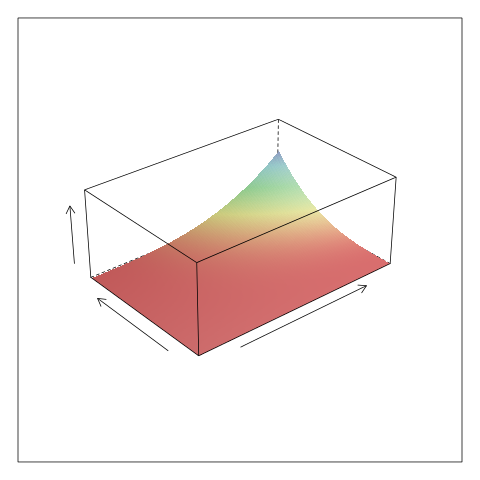
\includegraphics[width=.3\textwidth]{../FIGURES/EDD-ScaleFreeTrueGraphon} &
  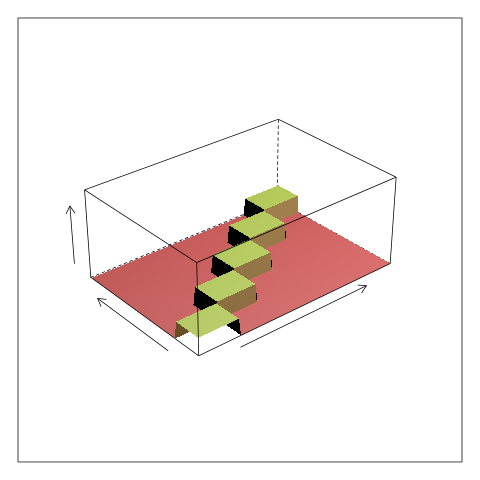
\includegraphics[width=.3\textwidth]{../FIGURES/CommunityTrueGraphon} &
  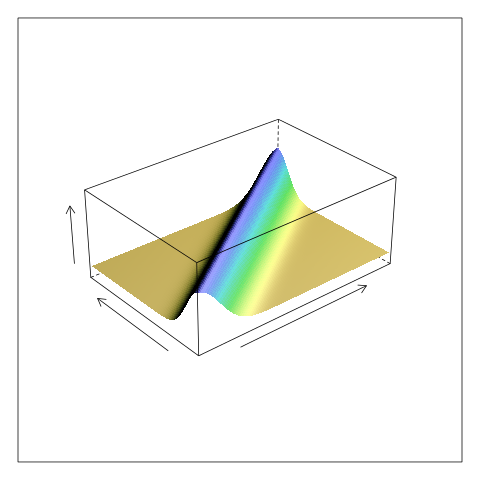
\includegraphics[width=.3\textwidth]{../FIGURES/SmallWorldTrueGraphon} 
  \end{tabular}
  } 
}

%====================================================================
\frame{\frametitle{Political blog network}

  $n = 196$ blogs ($N = 19110$ pairs), 3 covariates, density $= .075$ 

  \bigskip
  \begin{tabular}{cc}
    \begin{tabular}{p{.5\textwidth}}
	 Inferred graphon (no covariate) \\ ~\\
	 \includegraphics[height=.4\textheight]{../FIGURES/blogd0} \\ ~\\
	 ~
    \end{tabular}
    & 
    \hspace{-.05\textwidth}
    \begin{tabular}{p{.5\textwidth}}
	 Residual graphon (3 covariates) \\ ~\\
	 \includegraphics[height=.4\textheight]{../FIGURES/blogd3} \\ ~\\
	 $\Pt(H_0) \simeq 10^{-172}$
    \end{tabular}
  \end{tabular}
  }

%====================================================================
%====================================================================
\end{document}
%====================================================================
%====================================================================

  \begin{tabular}{cc}
    \begin{tabular}{p{.5\textwidth}}
    \end{tabular}
    & 
    \hspace{-.02\textwidth}
    \begin{tabular}{p{.5\textwidth}}
    \end{tabular}
  \end{tabular}
